\documentclass{beamer}

\usetheme{Padova}

\title{Esame di Laurea in Informatica}
\subtitle{Implementazione di modelli di programmazione matematica per problemi di bin packing}
\author{Daniel Rossi}
\date{18 Dicembre 2018}


\begin{document}

\maketitle

\begin{frame}{Outline}
	\tableofcontents
\end{frame}

\section{Introduzione}

\begin{frame}{Introduzione}
	\begin{minipage}[c]{0.45\textwidth}
		\large{\uppercase{Statistiche nazionali trasporti}} \vspace{.5em}
	\end{minipage}
	\hfill
	\begin{minipage}[c]{0.45\textwidth}
		
\includegraphics[width=\textwidth]{figures/logo}
	\end{minipage}
	\begin{block}{Logistica}
		7\% del PIL italiano
	\end{block}
	\begin{block}{Costi}
		11\% maggiore rispetto partner europei
	\end{block}
\end{frame}

\begin{frame}{Introduzione}
	\begin{block}{Tool aziendale}
		Euristica che dispone le merci nel container del camion
	\end{block}
	\begin{figure}[H]
		\begin{center} 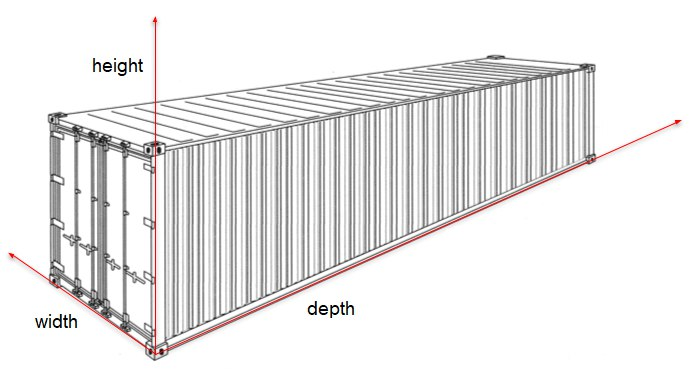
\includegraphics[scale=0.5]{figures/photo5805353100838547063}
		\end{center}
	\end{figure}
\end{frame}

\section{Proposta di stage}

\begin{frame}{Proposta di stage}
	\begin{alertblock}{Scopo}
		Lo scopo dello stage \`e  quello di realizzare dei modelli di programmazione lineare per la risoluzione dello \\ \textbf{Strip Packing Problem} da usare per valutare l'euristica aziendale
	\end{alertblock}
\end{frame}

\begin{frame}{Proposta di stage}
	\large{Obiettivi:}
	\begin{alertblock}{Realizzazione modelli:}
		\begin{itemize}
			\item \textbf{2D}: versione 2D;
			\item \textbf{2DR}: versione 2D con rotazione;
			\item \textbf{2DRS}: versione 2D con rotazione e sequenza di scarico;
			\item \textbf{3D}: versione 3D con rotazione e sovrapposizione.
		\end{itemize}
	\end{alertblock}
	\begin{alertblock}{Valutazione euristica:}
		\begin{itemize}
			\item Confronto delle soluzioni.
		\end{itemize}
	\end{alertblock}
\end{frame}
	
\section{Modelli matematici}
\begin{frame}{Modelli matematici}
		$$ max\; z = f ( x )\;\; (oppure\; min\; z = f ( x ))$$
		s.t.
		$$g_i (x) = \begin{cases} \leq b_i \\ = b_i, & i = 1,\dots,m \\ \geq b_i \end{cases}$$
		$$x = (x_1,\dots,x_n) \in X \subseteq \mathbb{R}^n$$
\end{frame}

\begin{frame}{Modello 2D}
	\begin{center}
		\begin{align*}
			& \underset{}{\text{min D}} \\
			  & \text{s.t.} &   & l_{ij} + l_{ji} + b_{ij} + b_{ji} \geq 1      & i < j    &   & i,j \in I \\
			  &             &   & y_i - y_j + M_d b_{ij} \leq M_d - d_i         &          &   & i,j \in I \\
			  &             &   & x_i - x_j + M_w l_{ij} \leq M_w - w_i         &          &   & i,j \in I \\
			  &             &   & x_i + w_i \leq W                              &          &   & i \in I   \\
			  &             &   & y_i + d_i \leq D                              &          &   & i \in I   \\
			  &             &   & b_{ij}, l_{ij} \in \{0,1\}                    & i \neq j &   & i,j \in I \\
			  &             &   & x_{i}, y_{i}, w_{i}, d_{i} \in \mathbb{R}^{+} &          &   & i \in I   
		\end{align*}
	\end{center}
	
\end{frame}

\end{document}
